Voici le document LaTeX avec la section « Certifications » retirée :

```latex
\documentclass{article}

\usepackage{times}
\usepackage{geometry}
\geometry{a4paper,left=0.6cm,right=0.7cm,top=2cm,bottom=1cm,columnsep=0.8cm}
\usepackage{fontawesome}
\usepackage[hidelinks]{hyperref}
\usepackage{multicol}
\usepackage{tikz}
\usepackage{hyphsubst}
\usepackage{moresize}
\usepackage{hyphenat}
\usepackage{tabularx}
\usepackage{xcolor}
\usepackage{enumitem}

\newcolumntype{Y}{>{\RaggedRight\arraybackslash}X}

\usepackage{enumitem}
\setlist[itemize]{itemsep=1pt,leftmargin=*,topsep=-10pt}

\definecolor{maincolor}{HTML}{f0fafc}
\definecolor{seccolor}{HTML}{ffffff}
\definecolor{gray}{HTML}{8c94a9}
\definecolor{sidetext}{HTML}{59cee5}

\usepackage[contents={}]{background}
\AddEverypageHook{\begin{tikzpicture}[remember picture,overlay]%
  \node[inner sep=0pt,outer sep=0pt] at (current page.north west) [anchor=north west]{%
  \fcolorbox{maincolor}{maincolor}{%
\begin{minipage}[t][\paperheight][t]{0.3\paperwidth}
        \color{white}
        \hspace{0.08cm}
\end{minipage}}
\fcolorbox{seccolor}{seccolor}{
\begin{minipage}[t][\paperheight][t]{0.67\paperwidth}
        \color{black}
        \hspace{1cm}
\end{minipage}
}
  };%
\end{tikzpicture}
}

\usepackage{enumitem}
\setlist[itemize]{itemsep=-2pt,topsep=0pt,leftmargin=1.08cm}
\renewcommand{\labelitemi}{\textcolor{sidetext}{\footnotesize$\bullet$}}

\setlength{\parindent}{0pt}
\usepackage{paracol}

\begin{document}

\pagestyle{empty}

\columnratio{0.3}
\begin{paracol}{2}
\color{sidetext}
\begin{center}
            \begin{tikzpicture}
            \clip (0,0) circle (1.5cm) node[anchor=center] {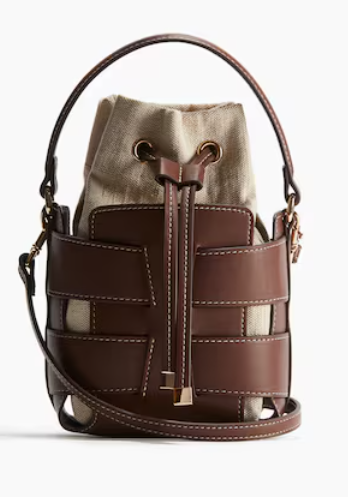
\includegraphics[width=3cm]{10058bbaa95b40d0968691ad70a631a2.png}}; 
            \end{tikzpicture}

            ~

         {\color{black}\LARGE \textbf{Pape Saliou FALL}}

         ~

         {\large{Data Scientist}}

        
        \end{center}

{\color{gray}\rule{\linewidth}{0.4pt}} \\

 \begin{tabular}{cl}
            \faPhone{}      & 
            \begin{tabular}{p{0.7\linewidth}}
            {\color{gray}Phone}\\
            {0753481453}
            \end{tabular}
            \\ \\
               \faLinkedin{}      & 
            \begin{tabular}{p{0.7\linewidth}}
            {\color{gray}LinkedIn}\\
            {\href{https://www.linkedin.com/in/pape}{https://www.linkedin.com/in/pape} }
            \end{tabular}
            \\ \\
               \faMapMarker{}      & 
            \begin{tabular}{p{0.7\linewidth}}
            {\color{gray}Address}\\
            {Paris, France}
            \end{tabular}
            \\ \\
               \faGlobe{}      & 
            \begin{tabular}{p{0.7\linewidth}}
            {\color{gray}Website/Blog}\\
            {\href{}{ }}
            \end{tabular}
            \\
        \end{tabular}
        \vspace{.2cm} \\
        {\color{gray}\rule{\linewidth}{0.4pt}} \\

        {\color{black}{Languages}}

        ~
        
        \begin{tabular}{cl}
            {\Large\faLanguage{}} & \begin{tabular}{l}
             {Français, Anglais} \\
             {\color{gray}Courant}
            \end{tabular} \\
        \end{tabular}
        \vspace{10pt} \\
        {\color{gray}\rule{\linewidth}{0.4pt}} \\

        \vspace{.4cm}

        {\color{black}{Key Skills}}

        ~
        
        \begin{tabular}{ll}
         \begin{minipage}{0.1\linewidth}
         
\includegraphics[width=\linewidth]{picon.png}
         \end{minipage} & Python \\[10pt]
         \begin{minipage}{0.1\linewidth}
         
\includegraphics[width=\linewidth]{picon.png}
         \end{minipage} & Machine Learning \\[10pt]
         \begin{minipage}{0.1\linewidth}
         
\includegraphics[width=\linewidth]{picon.png}
         \end{minipage} & SQL \\[10pt]
         \begin{minipage}{0.1\linewidth}
         
\includegraphics[width=\linewidth]{picon.png}
         \end{minipage} & AWS \\[10pt]
         \begin{minipage}{0.1\linewidth}
         
\includegraphics[width=\linewidth]{picon.png}
         \end{minipage} & Docker \\[10pt]
        \end{tabular}
        
\switchcolumn
\color{black}

\textcolor{black}{\Large \textbf{Professional Summary}} \\

\textcolor{black}{Data Scientist passionné par l’exploitation de la donnée pour créer de la valeur métier. Solide maîtrise de l’ensemble du cycle de vie des projets data : exploration, modélisation, industrialisation et suivi en production. Compétences approfondies en Machine Learning, statistiques et programmation (Python, R, SQL). Habitué à évoluer dans des environnements cloud (AWS) et à travailler en méthodologies agiles avec des équipes pluridisciplinaires.}\\[8pt]

\textcolor{black}{\Large \textbf{Work Experience}} \\

\colorbox{maincolor}{%
  \begin{minipage}{\linewidth}
    \begin{tabular}{@{}lp{0.72\linewidth}r}
      \begin{minipage}{0.05\linewidth}
        
\includegraphics[width=\linewidth]{picon.png}
      \end{minipage} & 
      Prepaya &  
      {\footnotesize 2022 -- 2023 } \\[-10pt]
      & {\color{sidetext}{Data Scientist}} & \\
      & {\small Paris, France } & \\
    \end{tabular}
\begin{itemize}
    \item Développé des modèles de prédiction de churn en Python (amélioration de 15 % du rappel)
\end{itemize}
  \end{minipage}%
}

~ \\[-6pt]

\colorbox{maincolor}{%
  \begin{minipage}{\linewidth}
    \begin{tabular}{@{}lp{0.72\linewidth}r}
      \begin{minipage}{0.05\linewidth}
        
\includegraphics[width=\linewidth]{picon.png}
      \end{minipage} & 
      Projet personnel open-source &  
      {\footnotesize 2021 -- Présent } \\[-10pt]
      & {\color{sidetext}{Développeur Data}} & \\
      & {\small } & \\
    \end{tabular}
\begin{itemize}
    \item Création d’outils de visualisation en Python, déployés sur Heroku et utilisés par 500+ utilisateurs mensuels
\end{itemize}
  \end{minipage}%
}


\vspace{1cm}

\textcolor{black}{\Large \textbf{Education}} \\


 \begin{tabular}{@{}cp{0.7\linewidth}}
      \begin{minipage}{0.05\linewidth}
        
\includegraphics[width=\linewidth]{picon.png}
      \end{minipage} & \vspace{-12pt}
      {\color{sidetext} {Master 2 Data Science}} \\[-6pt]
      & Sorbonne Université \\
      & Spécialité : Machine Learning \& Big Data \\
      & 2023 
    \end{tabular}


~

~

 \begin{tabular}{@{}cp{0.7\linewidth}}
      \begin{minipage}{0.05\linewidth}
        
\includegraphics[width=\linewidth]{picon.png}
      \end{minipage} & \vspace{-12pt}
      {\color{sidetext} {Licence Informatique}} \\[-6pt]
      & Université de Dakar \\
      & Informatique générale \\
      & 2021 
    \end{tabular}

% --- Section Certifications supprimée ---

\end{paracol}

\end{document}